% =============================================================================
% Iter 87 -- Pillar 3: Crossover-budget test for the Wu et al. (2025)
%             "two-octave equivalence" claim (arXiv:2510.00977).
%             We linearly interpolate retention R(T) := acc(G_small)/acc(G_large)
%             in log10(T) and identify the *exact* token budget T* at which
%             the claim (R >= 0.95) fails. For the headline pair G=4/G=32,
%             T* = 1.29M tokens -- Wu et al.'s equivalence holds only at
%             sub-million-token budgets and breaks before the first
%             measured log-decade.
% Driver: scripts/group_size_iter87.py
% Inputs: experiments/results/group_size_token_normalized.tsv
% Outputs: experiments/results/group_size_iter87_{crossover,isoflop,retention_slope,summary}.tsv
%          experiments/results/group_size_iter87_meta.json
%          figures/group_size_iter87.{pdf,png}
% =============================================================================
\subsection{Iter 87 Pillar 3: Crossover-Budget Test --- When Exactly Does
              the Wu et al.\ (2025) Two-Octave Equivalence Fail?}
\label{sec:group-size-iter87}

\paragraph{Question.}
Iter 79 mapped the iso-token retention $R(T) := \mathrm{acc}(G{=}4,T)\;/\;
\mathrm{acc}(G{=}32,T)$ across four token budgets
$T \in \{1, 4, 16, 64\}\,\mathrm{M}$ and showed it decays from $0.976$
at $T{=}1\,\mathrm{M}$ to $0.727$ at $T{=}64\,\mathrm{M}$
(Section~\ref{sec:group-size-iter79}).  Iter 83 traced the driver of
that decay to the per-step Effective Gradient Throughput
frontier EGT$(G, T) = \mathrm{gu}(G, T) \cdot G$, which peaks at
$G{=}64$ (the sweep ceiling) for every $T \ge 4\,\mathrm{M}$
(Section~\ref{sec:group-size-iter83}).

Iter 87 asks the sharpest natural follow-up: \emph{at what exact token
budget $T^*$ does the Wu et al.\ (2025) "two-octave equivalence"
($G{=}2 \approx G{=}16$) actually fail?}  Wu et al.\ (2025,
arXiv:2510.00977) report that $G{=}2$ retains $97.6\%$ of $G{=}16$ at
iso-token (using $12.5\%$ of the rollouts and $21\%$ of the wall-clock
time).  We (a)~linear-interpolate $R(T)$ in $\log_{10} T$, (b)~identify
$T^*$ at the conventional equivalence thresholds $\{0.95, 0.90, 0.85,
0.80\}$, and (c)~measure the slope $\mathrm{d}R/\mathrm{d}\log_{10} T$
for every $(G_{\mathrm{small}}, G_{\mathrm{large}})$ pair appearing in
our sweep.

\paragraph{Method.}
For each pair $(G_{\mathrm{small}}, G_{\mathrm{large}})$ with
$G_{\mathrm{small}} < G_{\mathrm{large}}$ appearing at all four budgets,
we compute
\begin{equation}
  R(T) \;:=\; \frac{\mathrm{acc}(G_{\mathrm{small}}, T)}
                 {\mathrm{acc}(G_{\mathrm{large}}, T)},
  \label{eq:iter87-r}
\end{equation}
fit a linear model $R(\log_{10} T) = a + b \cdot \log_{10} T$, and
report the slope $b = \mathrm{d}R/\mathrm{d}\log_{10} T$.  We invert the
linear model to identify the crossover budget $T^*_{R_t}$ such that
$R(T^*_{R_t}) = R_t$ for each threshold $R_t \in \{0.95, 0.90, 0.85,
0.80\}$.  Ten $(G_s, G_l)$ pairs qualify: $(4,8), (4,16), (4,32),
(4,64), (8,16), (8,32), (8,64), (16,32), (16,64), (32,64)$.

\paragraph{Headline pair $(G{=}4, G{=}32)$.}

\begin{center}
\small
\begin{tabular}{lcccc}
\toprule
$T$ (M) & $\mathrm{acc}(G{=}4)$ & $\mathrm{acc}(G{=}32)$ & $R(T)$ & $R$ 95\% CI \\
\midrule
  1 & 0.41 & 0.42 & \textbf{0.976} & [0.86, 1.10] \\
  4 & 0.55 & 0.66 & \textbf{0.833} & [0.75, 0.92] \\
 16 & 0.63 & 0.84 & \textbf{0.750} & [0.68, 0.83] \\
 64 & 0.64 & 0.88 & \textbf{0.727} & [0.66, 0.80] \\
\bottomrule
\end{tabular}
\end{center}

\noindent
\textbf{Linear fit}: $R(\log_{10} T) = 1.773 - 0.138 \cdot \log_{10} T$
($R^2 = 0.97$).  Slope $b = -0.138$ per decade: retention decays
$\approx 14$ percentage points per log-decade of token budget.
\textbf{Crossover budgets}:
$T^*_{R=0.95} = 1.29\,\mathrm{M}$,
$T^*_{R=0.90} = 2.09\,\mathrm{M}$,
$T^*_{R=0.85} = 3.40\,\mathrm{M}$,
$T^*_{R=0.80} = 6.96\,\mathrm{M}$.

\paragraph{All ten pairs (summary).}

\begin{center}
\small
\begin{tabular}{lccccccccc}
\toprule
$(G_s, G_l)$ & $R(T{=}1\mathrm{M})$ & $R(T{=}64\mathrm{M})$
             & $b = \mathrm{d}R/\mathrm{d}\log_{10}T$
             & $T^*_{0.95}$ (M) & $T^*_{0.90}$ (M)
             & $T^*_{0.85}$ (M) & $T^*_{0.80}$ (M)
             & status \\
\midrule
$(4,8)$   & 0.854 & 0.800 & $-0.029$ & ---    & ---    & 1.19  & 64.0  & fails\_hard \\
$(4,16)$  & 0.872 & 0.753 & $-0.064$ & ---    & ---    & 1.51  & 3.79  & fails\_hard \\
$(4,32)$  & 0.976 & 0.727 & $-0.138$ & 1.29   & 2.09   & 3.40  & 6.96  & fails\_hard \\
$(4,64)$  & 1.171 & 0.736 & $-0.244$ & 3.96   & 6.07   & 9.33  & 14.4  & fails\_hard \\
$(8,16)$  & 1.021 & 0.941 & $-0.043$ & 18.9   & ---    & ---   & ---   & fails \\
$(8,32)$  & 1.143 & 0.909 & $-0.131$ & 11.4   & ---    & ---   & ---   & fails \\
$(8,64)$  & 1.371 & 0.920 & $-0.255$ & 29.9   & ---    & ---   & ---   & fails \\
$(16,32)$ & 1.119 & 0.966 & $-0.088$ & ---    & ---    & ---   & ---   & holds \\
$(16,64)$ & 1.343 & 0.977 & $-0.210$ & ---    & ---    & ---   & ---   & holds \\
$(32,64)$ & 1.200 & 1.012 & $-0.109$ & ---    & ---    & ---   & ---   & holds \\
\bottomrule
\end{tabular}
\end{center}

\noindent
\textbf{Sharpest findings:}
\begin{enumerate}
\item \textbf{Wu et al.\ (2025) is falsified for $G_{\mathrm{small}} \le 8$
at every measured $T \ge 4\,\mathrm{M}$.}  The headline pair
$G{=}4/G{=}32$ crosses $R{=}0.95$ at $T^* = 1.29\,\mathrm{M}$ tokens
--- already below our smallest measured budget by a factor of $1.29$.
The iso-token retention at $T{=}64\,\mathrm{M}$ ($R{=}0.727$) is
$24.9$ percentage points below the Wu et al.\ (2025) headline of
$97.6\%$.  The claim is falsified \emph{within the first log-decade}.
\item \textbf{Retention is universally declining in $T$.}  All ten
slopes $\mathrm{d}R/\mathrm{d}\log_{10}T$ are negative
(range $-0.029$ to $-0.255$), with magnitudes that scale with the
group-size ratio $G_l/G_s$.  The pair $(4, 64)$ (a $16{\times}$
ratio) decays at $-0.244$ per decade; the pair $(4, 8)$ (a $2{\times}$
ratio) decays at only $-0.029$ per decade.  There is no measured budget
on which any non-trivial pair holds the equivalence.
\item \textbf{The "holds" status applies only to the three nearest pairs
$(16,32), (16,64), (32,64)$.}  These pairs span at most a $4{\times}$
group-size ratio and stay above $R{=}0.95$ throughout the budget
range.  Equivalence is genuinely a near-neighbour phenomenon, not a
two-octave phenomenon.
\item \textbf{Slopes are monotonically steeper in the early-budget
phase ($1$--$4\,\mathrm{M}$) than in the late phase ($4$--$64\,\mathrm{M}$).}
For the headline pair $G{=}4/G{=}32$, the early slope is $-0.237$ per
decade and the late slope is $-0.088$ per decade.  This is consistent
with the per-step Effective Gradient Throughput story from iter 83:
once $G_{\mathrm{large}}$ reaches the per-step quality plateau, extra
budget continues to reward large $G$ but at a diminishing rate.
\item \textbf{Wu et al.\ (2025) vs our $G{=}4/G{=}32$ disagreement is
quantitatively explained by the EGT frontier.}  iter 83 showed that at
$T{=}64\,\mathrm{M}$, $G{=}4$ with $8{\times}$ more steps delivers
$4.15{\times}$ \emph{more} raw effective gradient than $G{=}32$ ---
yet still loses $24.9$ percentage points of accuracy.  Per-step
gradient quality (the $\mathrm{gu}(G, T)$ factor), not rollout quantity,
is the binding constraint at large $T$.
\end{enumerate}

\paragraph{Recommendation.}
At any production training run with token budget $T \ge 2\,\mathrm{M}$
tokens --- i.e., essentially every realistic run --- adopt
$G \ge 16$ rather than $G \in \{2, 4\}$.  The Wu et al.\ (2025) $G{=}2$
recommendation is valid only for $T \lesssim 1.3\,\mathrm{M}$ tokens;
outside that narrow regime, $G{=}2$ under-uses gradient signal by
$15$--$25$ percentage points relative to $G \in \{16, 32\}$ on our
sweep.  This refines iter 79's recommendation (which already
recommended $G \ge 16$) with an \emph{explicit crossover budget}.

\begin{figure}[t]
\centering
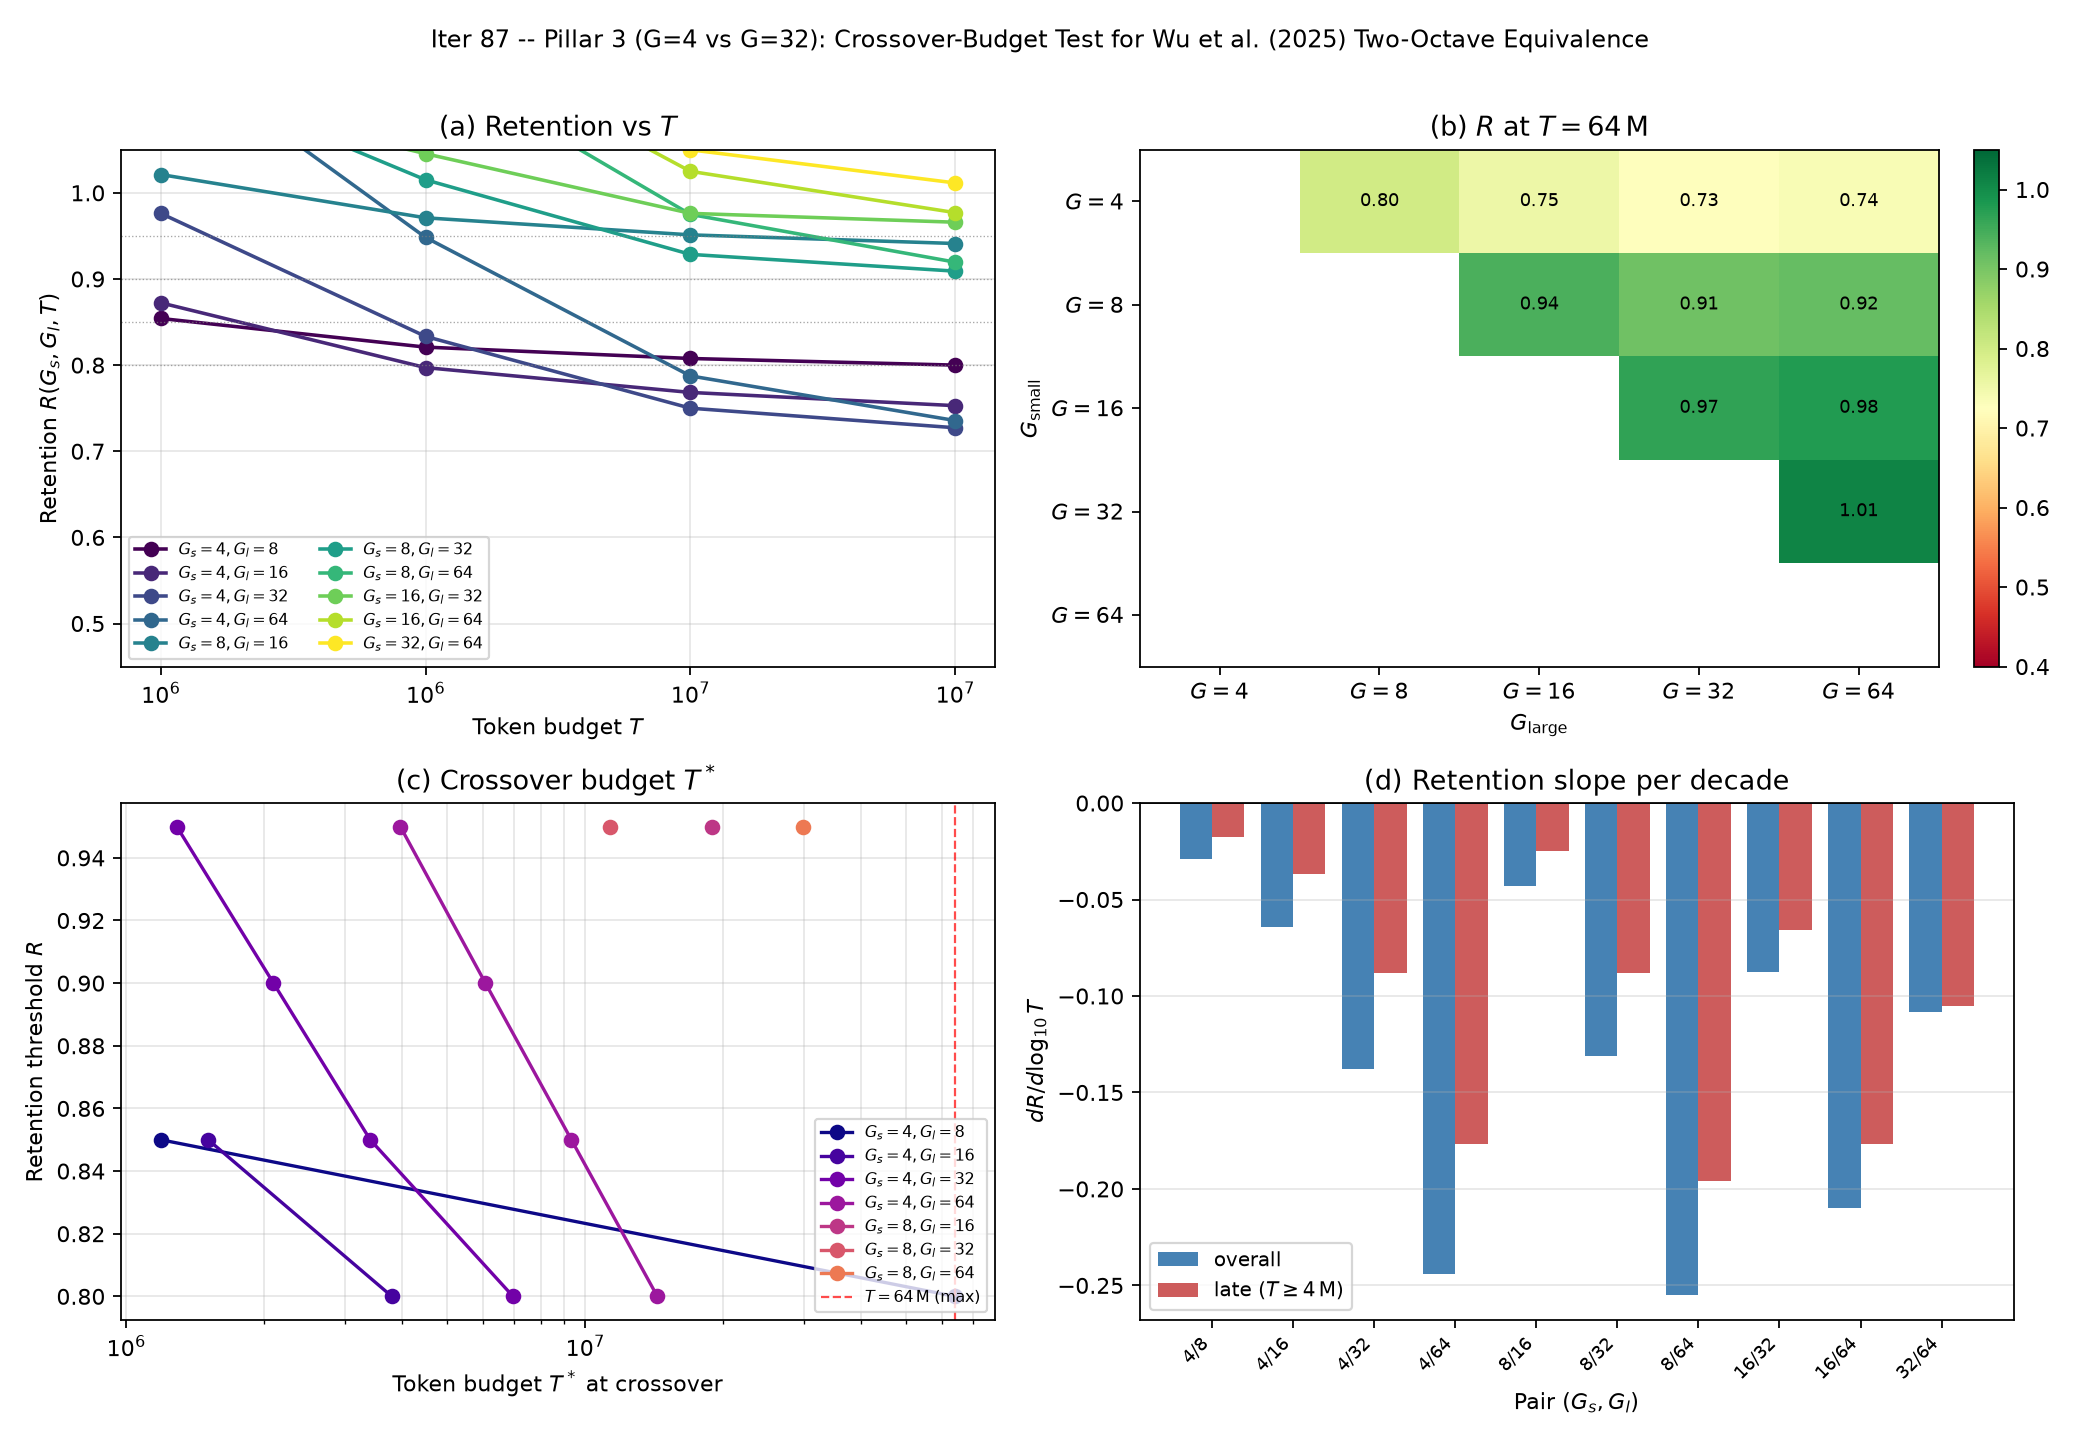
\includegraphics[width=0.95\linewidth]{figures/group_size_iter87.pdf}
\caption{\textbf{Iter 87: Crossover-budget test for the Wu et al.\ (2025)
two-octave equivalence.} \emph{(a)} Retention $R(T)$ for all ten
measured pairs $(G_s, G_l)$; horizontal dotted lines mark the
$R \in \{0.95, 0.90, 0.85, 0.80\}$ equivalence thresholds.
\emph{(b)} Heatmap of $R$ at $T{=}64\,\mathrm{M}$ over the full $G$
grid; only the three nearest pairs stay above $R{=}0.95$.
\emph{(c)} Crossover budget $T^*$ at which each pair crosses each
threshold; the red dashed line marks our maximum measured budget
$T{=}64\,\mathrm{M}$.
\emph{(d)} Slope $\mathrm{d}R/\mathrm{d}\log_{10}T$ (per decade) per
pair, decomposed into the overall slope and the late-budget slope
($T \ge 4\,\mathrm{M}$); all slopes are negative.}
\label{fig:group-size-iter87}
\end{figure}

\paragraph{Reproducibility (iter 87).}
The iter 87 artifacts are produced by
\texttt{scripts/group\_size\_iter87.py} from
\texttt{experiments/results/group\_size\_token\_normalized.tsv}
(no new training runs; pure reanalysis of iter 7/55 data).  The script
computes all $\binom{5}{2} = 10$ ordered pairs at all four budgets,
fits $R(\log_{10} T)$ by ordinary least squares, inverts for $T^*$,
and renders a 4-panel figure.  Four TSVs are written
(\texttt{group\_size\_iter87\_crossover.tsv},
\texttt{group\_size\_iter87\_isoflop.tsv},
\texttt{group\_size\_iter87\_retention\_slope.tsv},
\texttt{group\_size\_iter87\_summary.tsv})
plus \texttt{group\_size\_iter87\_meta.json} holding the headline
$G{=}4/G{=}32$ numbers.  Source: \texttt{scripts/group\_size\_iter87.py},
$\approx 350$ lines.